\documentclass{article}
\usepackage[utf8]{inputenc}
\usepackage{amsmath}
\usepackage{amsfonts}
\usepackage{amsthm}
\usepackage{amssymb}
\usepackage{systeme}
\usepackage{graphicx}

\setlength{\parindent}{0em}
\setlength{\parskip}{1em}

\title{Homework 6}
\author{Jackson Hart}
\date{February 25, 2022}

\begin{document}

\maketitle
\section*{Problem 1}
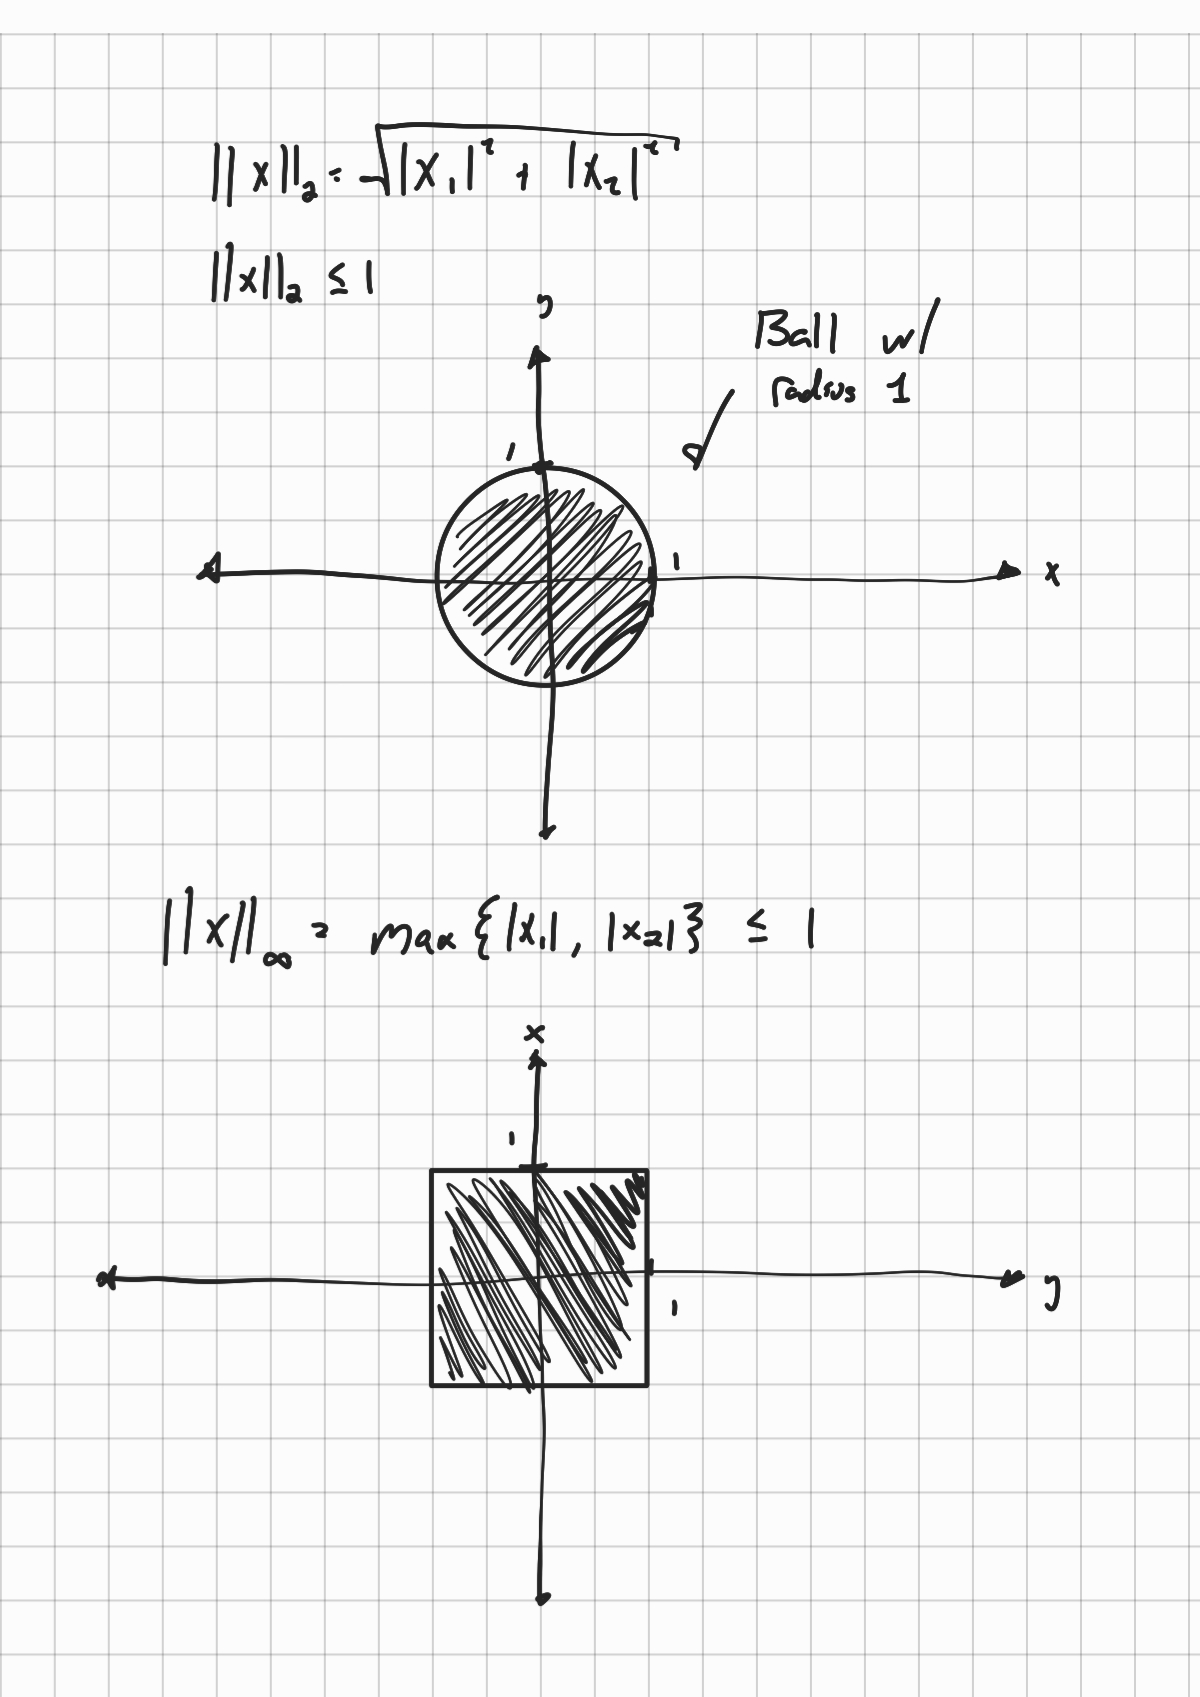
\includegraphics[scale=0.25]{Temp}

\section*{Problem 2}
Suppose $P: V \rightarrow V$ satisfies both $P^* = P$ and $P^2 = P$. Then $P$ is an orthogonal projection onto $Ran(P)$.
\begin{proof}
An orthogonal projection is defined as $P_Ev = w$ such that $w \in E$ and $v-w \perp E$. In this case, $E = Ran(P)$. By definition of range, we know the first condition to be true. For the second condition, we must consider $x \in V$, $y \in Ran(P)$ such that $Px = y$, and another arbitrary vector $z \in Ran(P)$. So, 

\[ \langle x - y, z \rangle \]

Because $z \in Ran(P)$, $\exists v \in V$ such that $Pv = z$. So,

\[ \langle x - Px, Pv \rangle \]
\[ = \langle x, Pv \rangle - \langle Px, Pv \rangle \]
\[ = \langle x, Pv \rangle - \langle x, P^*Pv \rangle \]
\[ = \langle x, Pv \rangle - \langle x, P^2v \rangle \]
\[ = \langle x, Pv \rangle - \langle x, Pv \rangle \]
\[ \langle x, Pv \rangle = \langle x, Pv \rangle  \]

Because these two inner products equal each other, we can then say that

\[ \langle x, pv \rangle - \langle Px, Pv \rangle = 0 \]
\[ => \langle x - y, z \rangle = 0 \]

So therefore, $x - y \perp z$. Because $z$ is an arbitrary vector $\in Ran(P)$, this then works for all vectors $\in Ran(P)$, so therefore, $x - y \perp Ran(P)$. So therefore, $P$ is an orthogonal projection onto $Ran(P)$. 

\end{proof}

\section*{Problem 3}
Let $\mathcal{B} = \{v_1, ..., v_n\}$ be an orthonormal basis in $V$.
\subsection*{A}
For any $x = \sum_{k=1}^{n}\alpha_k v_k$ and $y = \sum_{k=1}^{n}\alpha_k v_k$, we have that

\[ \langle x, y \rangle = \sum_{k=1}^{n} \alpha_k \overline{\beta_k} \]

\begin{proof}
Consider,

\[ \langle x, y \rangle = \langle \sum^n_{k=1} \alpha_k v_k, y \rangle \] 
\[ = \sum^n_{k=1} \alpha_k \langle v_k, y \rangle \]
\[ = \sum^n_{k=1} \alpha_k \langle v_k, \sum^n_{j=1} \beta_j v_j \rangle \]
\[ = \sum^n_{k=1} \sum^n_{j=1} \alpha_k \overline{\beta_j} \langle v_k, v_j \rangle \]

Now, because $v_k, v_j \in \mathcal{B}$ and $\mathcal{B}$ is an orthonormal basis, $v_k$ and $v_j$ are orthogonal to each other, so $\langle v_k, v_j \rangle = 0$. Except in the case that $v_k = v_j$, in which case, $\langle v_k, v_j \rangle = 1$. So the value inside the summation is equal to $\alpha_k \beta_j$ only where $k = j$, so,

\[ \sum^n_{k=1} \sum^n_{j=1} \alpha_k \overline{\beta_j} \langle v_k, v_j \rangle = \sum_{k=1}^n \alpha_k \overline{\beta_k} \]

\end{proof} 

\subsection*{B}
Consider $\langle x, v_k \rangle$. Based on the formula found in the last problem, we know that

\[ \sum^n_{k=1} \langle x, v_k \rangle = \sum^n_{k=1} \alpha_k * 1 \]

Now consider $\langle v_k, y \rangle$. Again,

\[ \sum^n_{k=1} \langle v_k, y \rangle = \sum^n_{k=1} \overline{\langle y, v_k \rangle} = \sum^n_{k=1} \overline{\beta_k} * 1 \]

So then we can say,

\[ \sum^n_{k=1} \langle x, v_k \rangle \langle v_k, y \rangle = \sum^n_{k=1} \alpha_k \overline{\beta_k} = \langle x, y \rangle \]

\[ \therefore \langle x, y \rangle = \sum^n_{k=1} \langle x, v_k \rangle \overline{ \langle y, v_k \rangle} \]

\section*{Problem 4}
Let $x_1 = \begin{bmatrix} 1 \\ 1 \\ 0 \end{bmatrix}$, $x_2 = \begin{bmatrix} 2 \\ 0 \\ 1 \end{bmatrix}$, and $x_3 = \begin{bmatrix} 2 \\ 2 \\ 1 \end{bmatrix}$. Define $\{v_1, v_2, v_3\}$ as an orthogonal set with the same span as $\{x_1, x_2, x_3\}$. Let $v_1 = x_1$. Then,

\[ v_2 = \begin{bmatrix} 2 \\ 0 \\ 1 \end{bmatrix} - \frac{<2, 0, 1> \cdot <1, 1, 0>}{||<1, 1, 0>||^2} \begin{bmatrix} 1 \\ 1 \\ 0 \end{bmatrix} \]
\[ v_2 = \begin{bmatrix} 2 \\ 0 \\ 1 \end{bmatrix} - \frac{2}{2} \begin{bmatrix} 1 \\ 1 \\ 0 \end{bmatrix} \]
\[ v_2 = \begin{bmatrix} 1 \\ -1 \\ 1 \end{bmatrix} \]

\[ v_3 = \begin{bmatrix} 2 \\ 2 \\ 1 \end{bmatrix} - \frac{<2, 2, 1> \cdot <1, 1, 0>} {||<1, 1, 0>||^2} \begin{bmatrix} 1 \\ 1 \\ 0 \end{bmatrix} - \frac{<2, 2, 1> \cdot <1, -1, 1>}{||<1, -1, 1>||^2} \begin{bmatrix} 1 \\ -1 \\ 1 \end{bmatrix} \]
\[ v_3 = \begin{bmatrix} 2 \\ 2 \\ 1 \end{bmatrix} - \frac{4}{2} \begin{bmatrix} 1 \\ 1 \\ 0 \end{bmatrix} - \frac{1}{3} \begin{bmatrix} 1 \\ -1 \\ 1 \end{bmatrix} \]
\[ v_3 = \begin{bmatrix} 2 \\ 2 \\ 1 \end{bmatrix} - \begin{bmatrix} 2 \\ 2 \\ 0 \end{bmatrix} - \begin{bmatrix} \frac{1}{3} \\ -\frac{1}{3} \\ \frac{1}{3} \end{bmatrix} \]
\[ v_3 = \begin{bmatrix} -\frac{1}{3} \\ \frac{1}{3} \\ \frac{2}{3} \end{bmatrix} \]

This set is orthogonal, but to also make them normal,

\[ \text{let } v_1 = \frac{\begin{bmatrix} 1 & 1 & 0 \end{bmatrix}^T}{||<1, 1, 0>||} \]
\[ v_1 = \frac{1}{\sqrt{2}} \begin{bmatrix} 1 \\ 1 \\ 0 \end{bmatrix} \]

\[ \text{let } v_2 = \frac{\begin{bmatrix} 1 & -1 & 1 \end{bmatrix}^T}{||<1, -1, 1>||} \]
\[ v_2 = \frac{1}{\sqrt{3}} \begin{bmatrix} 1 \\ -1 \\ 1 \end{bmatrix} \]

\[ \text{let } v_3 = \frac{\frac{1}{3} \begin{bmatrix} -1 & 1 & 2 \end{bmatrix}^T}{||\frac{1}{3}<-1, 1, 2>||} \]
\[ v_3 = \frac{1}{3 \sqrt{3}} \begin{bmatrix} -1 \\ 1 \\ 2 \end{bmatrix} \]

\section*{Problem 5}
Let $W$ be a finite-dimensional subspace of an inner product space $V$. If $P$ is orthogonal projection onto $W$, then $I - P$ is orthogonal projection onto $W^\perp$.

\begin{proof}
Let $v \in V$ be such that $Pv \in W$. We know that by definition of an orthogonal projection, $v - Pv \in W^{\perp}$. So consider,

\[ (I - P)v \]
\[ => v - Pv \]

So therefore, $(I - P) \in W^{\perp}$, so $I - P$ fulfills the first property of the definition of orthogonal projection. Now,

\[ v - (I - P)v \]
\[ v - v - Pv \]
\[ (v - Pv) \perp W^{\perp} \]

Which satisfies the second property of the definition of orthogonal projection.
\end{proof}

\section*{Problem 6}
Let $A \in M_{nxn}(\mathbb{F})$. $ker(A^*A + I) = \{ 0 \}$. 

\begin{proof}
Let $v$ be an arbitrary vector $\in ker(A^*A + I)$. Then, $(A^*A + I)v = 0$, so

\[ \langle (A^*A + I)v, v \rangle = 0 \]
\[ => \langle A^*Av + Iv, v \rangle = 0 \]
\[ => \langle A^*Av, v \rangle + ||v||^2 = 0 \]
\[ => \langle Av, Av \rangle + ||v||^2 = 0 \]

\[ ||Av||^2 + ||v||^2 = 0 \]

By the inner product's non-negativity property, $||Av||^2 \ge 0$ and $||v||^2 \ge 0$, so therefore,

\[ ||v|| = 0 \]
\[ \text{so } v = 0 \text{ by non-degeneracy} \]

\end{proof}

\end{document}